% Adjust these for the path of the theme and its graphics, relative to this file
%\usepackage{beamerthemeFalmouthGamesAcademy}
\usepackage{../../beamerthemeFalmouthGamesAcademy}
\usepackage{multimedia}
\graphicspath{ {../../} }
\newcommand{\modulecode}{COMP260}\newcommand{\moduletitle}{Distributed Systems}\newcommand{\sessionnumber}{5}

% Default language for code listings
\lstset{language=C++,
        morekeywords={each,in,nullptr}
}
\hypersetup{
    colorlinks=true,
    linkcolor=white,
    filecolor=magenta,      
    urlcolor=cyan,
}

% For strikethrough effect
\usepackage[normalem]{ulem}
\usepackage{wasysym}
\usepackage{gensymb}
\usepackage{pdfpages}
\usepackage{verbatim}
\usepackage{longtable,booktabs}

\usepackage{lmodern}
\usepackage{amssymb,amsmath}
\usepackage{ifxetex,ifluatex}
\usepackage{fixltx2e} % provides \textsubscript
\ifnum 0\ifxetex 1\fi\ifluatex 1\fi=0 % if pdftex
  \usepackage[T1]{fontenc}
  \usepackage[utf8]{inputenc}
\else % if luatex or xelatex
  \ifxetex
    \usepackage{mathspec}
  \else
    \usepackage{fontspec}
  \fi
  \defaultfontfeatures{Ligatures=TeX,Scale=MatchLowercase}
\fi
% use upquote if available, for straight quotes in verbatim environments
\IfFileExists{upquote.sty}{\usepackage{upquote}}{}
% use microtype if available
\IfFileExists{microtype.sty}{%
\usepackage{microtype}
\UseMicrotypeSet[protrusion]{basicmath} % disable protrusion for tt fonts
}{}
\newif\ifbibliography
\hypersetup{
            pdftitle={test},
            pdfauthor={Al},
            pdfborder={0 0 0},
            breaklinks=true}
\urlstyle{same}  % don't use monospace font for urls
\usepackage{longtable,booktabs}
\usepackage{caption}
% These lines are needed to make table captions work with longtable:
\makeatletter
\def\fnum@table{\tablename~\thetable}
\makeatother
\usepackage{graphicx,grffile}
\makeatletter
\def\maxwidth{\ifdim\Gin@nat@width>\linewidth\linewidth\else\Gin@nat@width\fi}
\def\maxheight{\ifdim\Gin@nat@height>\textheight0.8\textheight\else\Gin@nat@height\fi}
\makeatother
% Scale images if necessary, so that they will not overflow the page
% margins by default, and it is still possible to overwrite the defaults
% using explicit options in \includegraphics[width, height, ...]{}
\setkeys{Gin}{width=\maxwidth,height=\maxheight,keepaspectratio}

% Prevent slide breaks in the middle of a paragraph:
\widowpenalties 1 10000
\raggedbottom

\AtBeginPart{
  \let\insertpartnumber\relax
  \let\partname\relax
  \frame{\partpage}
}
\AtBeginSection{
  \ifbibliography
  \else
    \let\insertsectionnumber\relax
    \let\sectionname\relax
    \frame{\sectionpage}
  \fi
}
\AtBeginSubsection{
  \let\insertsubsectionnumber\relax
  \let\subsectionname\relax
  \frame{\subsectionpage}
}

\setlength{\parindent}{0pt}
\setlength{\parskip}{6pt plus 2pt minus 1pt}
\setlength{\emergencystretch}{3em}  % prevent overfull lines
\providecommand{\tightlist}{%
  \setlength{\itemsep}{0pt}\setlength{\parskip}{0pt}}
\setcounter{secnumdepth}{0}

% http://www.texample.net/tikz/examples/state-machine/
\usetikzlibrary{arrows,automata}

\providecommand{\tightlist}{%
  \setlength{\itemsep}{0pt}\setlength{\parskip}{0pt}}



\begin{document}
\title{\sessionnumber: Data Collection for Evaluating Interfaces \& Interactions}
\subtitle{\modulecode: \moduletitle}

\frame{\titlepage} 

% ----------------------------------------------- Generated with RMarkdown (Experimental)------------------------------------------------- %


\section{Session 2: Data Collection for Evaluating Interfaces \&
Interactions}\label{session-2-data-collection-for-evaluating-interfaces-interactions}

\begin{frame}{Register Attendance}

\begin{figure}
\centering
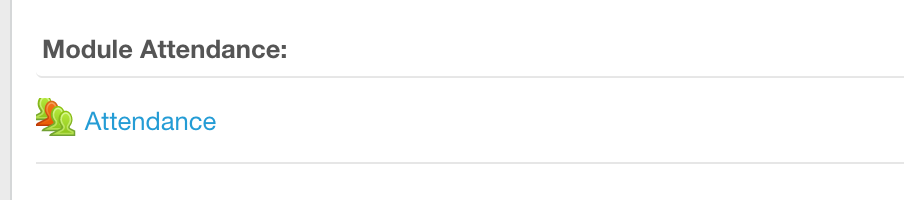
\includegraphics{assets/attendance.png}
\caption{Attendance monitoring is in place. It is your responsability to
ensure that you have signed yourself in.}
\end{figure}

\end{frame}

\begin{frame}{Learning Outcomes}

\begin{itemize}
\tightlist
\item
  \textbf{Select} the right participants for a HCI study
\item
  \textbf{Consider} the participants needs
\item
  \textbf{Conduct} Interviews and focus groups correctly
\end{itemize}

\end{frame}

\subsection{Human Subjects - Human
Considerations}\label{human-subjects---human-considerations}

\begin{frame}{Who?}

\begin{itemize}
\tightlist
\item
  Is the system designed for experts or more general users?
\item
  Are the participants the independent variable? (age, gender, height)
\end{itemize}

\textbf{General}

\begin{itemize}
\tightlist
\item
  Appropriateness / Target Audience
\item
  Individual's goals, background and motivations
\item
  Technical Competency
\item
  Gender
\end{itemize}

Gaming Specific - Gaming Expertise - Gaming Preferences

\end{frame}

\begin{frame}{Numbers}

\begin{itemize}
\tightlist
\item
  Cost vs benefit
\item
  Time required per participant
\item
  Dependent on the type of research and design of the study
\item
  Cook \& Campbell - Classic Reading
  \href{https://moodle2.units.it/pluginfile.php/132646/mod_resource/content/1/Estratto_ShadishCookCampbellExperimental2002.pdf}{{[}Find
  it here{]}}
\end{itemize}

\end{frame}

\begin{frame}{Large Numbers}

\begin{itemize}
\tightlist
\item
  Usually involve a diverse range of participants
\item
  Outcome is separate from the individuals
\item
  Expensive
\item
  Complex
\end{itemize}

\end{frame}

\begin{frame}{Small Numbers}

\begin{itemize}
\tightlist
\item
  More participants = More statistical power
\item
  Usability Test - 5 people are enough? (Nielsen \& Molich 1990)
\item
  Studies with 12 participants are not uncommon
\item
  20+ are better
\end{itemize}

\end{frame}

\begin{frame}{Individual}

\begin{itemize}
\tightlist
\item
  Inexpensive
\item
  Limited
\item
  Non-representative
\item
  Not statistically significant
\item
  Helpful on a personal level - auto ethnography
\end{itemize}

\end{frame}

\begin{frame}{Recruitment}

\begin{itemize}
\tightlist
\item
  Dependent on Study
\item
  Games Academy FTW
\item
  GDPR
\item
  Commensurate Incentivisation (pizza ++)
\item
  Over-recruit if you can
\end{itemize}

\end{frame}

\begin{frame}{Protecting the Participant}

\begin{itemize}
\item
  Informed Consent (Usually, a signed form)
\item
  Respect and Trust
\item
  Respect for the individual, beneficence (moral obligation) and justice
  (benefits are for all and not just one privileged group) (National
  Commission for the protection of Human Subjects of Biomedical and
  Behavioural Research, 1979)
\item
  Privacy

  \begin{itemize}
  \tightlist
  \item
    Image and video - Protect identities where possible
  \item
    Data Storage (GDPR again!)
  \item
    Consider Dissemination throughout
  \end{itemize}
\end{itemize}

\end{frame}

\begin{frame}{Institutional Review Boards (IRB)}

\begin{itemize}
\tightlist
\item
  Most institutions that engage in research have an ethics review board
\item
  Approval is needed to begin the research (NOT IN THIS MODULE)
\item
  Falmouth University Policy can be found
  \href{https://www.falmouth.ac.uk/sites/default/files/download/research_ethics_policy-13nov15.pdf}{HERE}
\end{itemize}

\end{frame}

\begin{frame}{Qualitative, Quantitative \& Mixed Method}

\begin{itemize}
\tightlist
\item
  \textbf{Qualitative:} (qual) data, collects information that seeks to
  describe a topic more than measure it. Think of impressions, opinions,
  and views. A qualitative survey is less structured: It seeks to delve
  deep into the topic at hand to gain information about people's
  motivations, thinking, and attitudes. While this brings depth of
  understanding to your research questions, it also makes the results
  harder to analyze.
\item
  \textbf{Quantitative:} (quant) data is designed to collect cold, hard
  facts. Numbers. Quantitative data is structured and statistical. It
  provides support when you need to draw general conclusions from your
  research.
  \href{https://www.surveymonkey.com/mp/quantitative-vs-qualitative-research/}{(source)}
\item
  \textbf{Mixed Method:} A study that combines the
  two\href{http://didier-jourdan.com/wp-content/uploads/2017/04/MM-and-Graduates-students.pdf}{(Useful
  reading)}
\end{itemize}

\end{frame}

\begin{frame}{User Research Methods}

\begin{longtable}[]{@{}ll@{}}
\toprule
Qualitative & Quantitative\tabularnewline
\midrule
\endhead
Interviews & Automated Data Collection\tabularnewline
Focus Groups & Physiological Data\tabularnewline
Diaries & Eye Tracking\tabularnewline
Camera Study & Task Analysis\tabularnewline
Surveys & A/B testing\tabularnewline
Heuristic Evaluation & Bench Marking\tabularnewline
Cognitive Walkthroughs & Surveys\tabularnewline
Ethnographic Field Study & Click Stream Analysis\tabularnewline
Think Aloud Protocol & System Usability Scale (SUS)\footnote<.->{More
  information on SUS can be found
  \href{https://moodle2.units.it/pluginfile.php/132646/mod_resource/content/1/Estratto_ShadishCookCampbellExperimental2002.pdf}{here}}\tabularnewline
\bottomrule
\end{longtable}

\end{frame}

\section{Surveys}\label{surveys}

\begin{frame}{What is a Survey?}

\begin{quote}
``In short, it is a well defined and well-written set of questions to
which an individual is asked to respond''
\end{quote}

(Lazar et al., 2017)

\begin{itemize}
\tightlist
\item
  Often used, hardly ever done well
\item
  Easy to generate data that is not relevant or valid
\item
  Misconceived as easy
\item
  Require pilot test
\item
  Good for measuring attitudes, awareness, intent, and getting feedback
\end{itemize}

\end{frame}

\begin{frame}{Pros \& Cons}

\begin{longtable}[]{@{}ll@{}}
\toprule
Pros & Cons\tabularnewline
\midrule
\endhead
Large Sample Groups & Hard to refine\tabularnewline
Low Cost & No follow-up questions\tabularnewline
Help to understand a population & Shallow understanding\tabularnewline
Distributed Easily &\tabularnewline
Easy to get approval &\tabularnewline
Good for factual information & Suffer from recall bias \footnote<.->{\href{https://en.wikipedia.org/wiki/Recall_bias}{Recall
  Bias}}\tabularnewline
\bottomrule
\end{longtable}

\end{frame}

\begin{frame}{Question Design}

Questions must be:

\begin{itemize}
\tightlist
\item
  balanced \& non biased
\item
  Easy to understand by the participant
\end{itemize}

There are three main types of question.

\begin{itemize}
\tightlist
\item
  Open-ended
\item
  Closed-ended - ordered response
\item
  Closed-ended - unordered response
\end{itemize}

\end{frame}

\begin{frame}{Open-Ended}

\begin{quote}
``Open-ended questions are useful for getting a better understanding of
phenomena, because they give the respondant complete flexibility in
their answers''
\end{quote}

(Lazar et al., 2017)

\textbf{Considerations}

\begin{itemize}
\tightlist
\item
  Extra care is needed to extract the right information
\item
  Provide sufficient detail
\item
  Avoid ambiguity
\end{itemize}

\end{frame}

\begin{frame}

\textbf{Bad:} How did you feel about the drop-down menu interface?

\textbf{Good:} list the issues you faced when trying to navigate using
the drop-down menu interface?

More specific to the needs of the study.

\end{frame}

\begin{frame}{Closed-Ended}

Closed ended questions constrain the users answers within a range of
choices designed by you.

\begin{itemize}
\tightlist
\item
  \textbf{Ordered:} one of more answers can be selected in some logical
  order.
\item
  \textbf{Unordered:} One or more answer can be selected with no
  relationship between each other.
\end{itemize}

\end{frame}

\begin{frame}{}

\begin{figure}
\centering
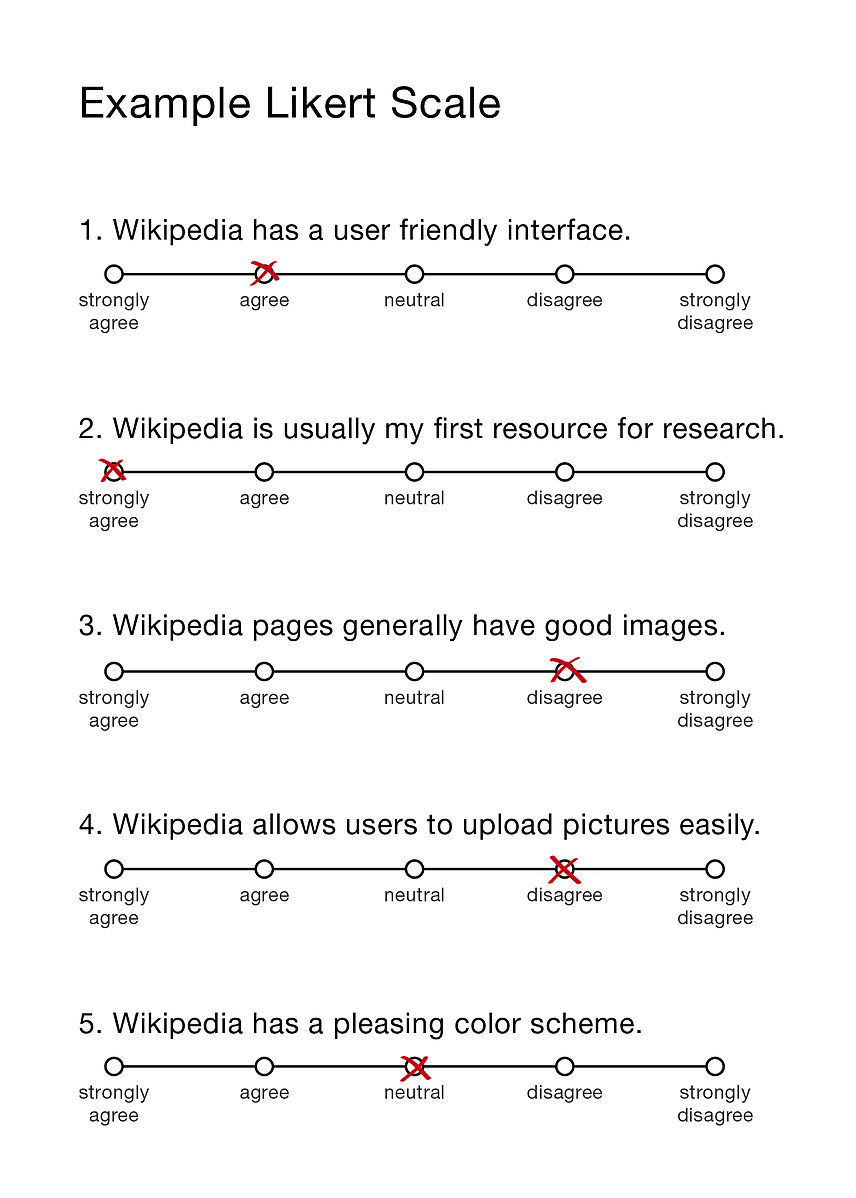
\includegraphics{assets/likert.jpg}
\caption{One example of closed-ended ordered response questions is the
Likert Scale}
\end{figure}

\end{frame}

\begin{frame}{Sampling}

A census is generally considered impossible. Instead, we do
probabilistic (random) sampling. This gives us a general picture of the
attitudes or feeling of a certain population.

\textbf{EXAMPLE}

In a study designed to gauge student attitudes towards food served in
the Stannary, it would be unrealistic to expect to reach out to every
student (5000+) and achieve a 100\% response rate. Instead, you might
take a random slice of 10\%.

\end{frame}

\begin{frame}{Targeted Users}

\begin{itemize}
\tightlist
\item
  Consider the targeted respondents
\item
  Set clear Limits (inclusion/exclusion criteria)
\item
  Identify communities of interest
\item
  Decide on a dissemination plan
\end{itemize}

\end{frame}

\begin{frame}{Pilot Test}

\textbf{DO NOT} release a survey into the wild without running some
pretesting!

\begin{itemize}
\tightlist
\item
  Review: Get the the survey checked by other experts
\item
  Test: Find a very small sample 3-5 and run hybrid interviews
\item
  Pilot: release the survey to a small test sample
\end{itemize}

The pilot study can be the difference between useful data and nonsense!

\end{frame}

\begin{frame}{\color<1>[rgb]{1,0,0} Common Mistakes}

\begin{itemize}
\tightlist
\item
  Double Barreled Question
\item
  Bias/loaded words (avoid overly negative or positive sounds words)
\item
  Provocative language such as ``liberal'', ``terrorism'',
  ``conservative''\ldots{}
\item
  Assuming prior knowledge
\item
  Inadequate response options (frustrate the user)
\item
  Lengthy survey
\end{itemize}

\end{frame}

\begin{frame}{Overall Survey Design}

\begin{itemize}
\tightlist
\item
  It is useful to be explicit about the inclusion criteria within the
  survey
\item
  grouping is helpful
\item
  Questions don't exist in a vacuum
\item
  Order and flow is important
\item
  keep it as short as possible
\item
  Place sensitive questions towards the end of the survey
\item
  Always provice attribution so the participant knows who you are and
  how to contact you
\end{itemize}

\end{frame}

\begin{frame}{Why Reinvent the Wheel?}

Find an existing tool and apply it to your study. You may need to modify
the questions to better suit your goals.

\begin{itemize}
\tightlist
\item
  Computer System Usability Questionnaire (CSUQ)
\item
  Interface Consistency Testing Questionnaire (ICTQ)
\item
  Perdue Usability Testing Questionnaire (PUTQ)
\item
  Questionnaire for User Interaction Satisfaction (QUIS)
\item
  Software Usability Measurement Inventory (SUMI)
\item
  System Usability Scale (SUS)
\end{itemize}

Always check the validity of existing surveys through peer reviewed
evaluation before utilising it in your own study!

\end{frame}

\end{document}


